\documentclass{article}

\usepackage{graphicx}
\usepackage{tikz}
\usepackage{tikzsymbols}
\usetikzlibrary{calc,patterns,shapes.geometric}
\pagestyle{empty}
\usepackage[margin=0pt]{geometry}
\geometry{papersize={14in,12in}}

\def\centerarc[#1](#2)(#3:#4:#5){\draw[#1] ($(#2)+({#5*cos(#3)},{#5*sin(#3)})$) arc (#3:#4:#5);}

\begin{document}
	\begin{figure}
		\centering
		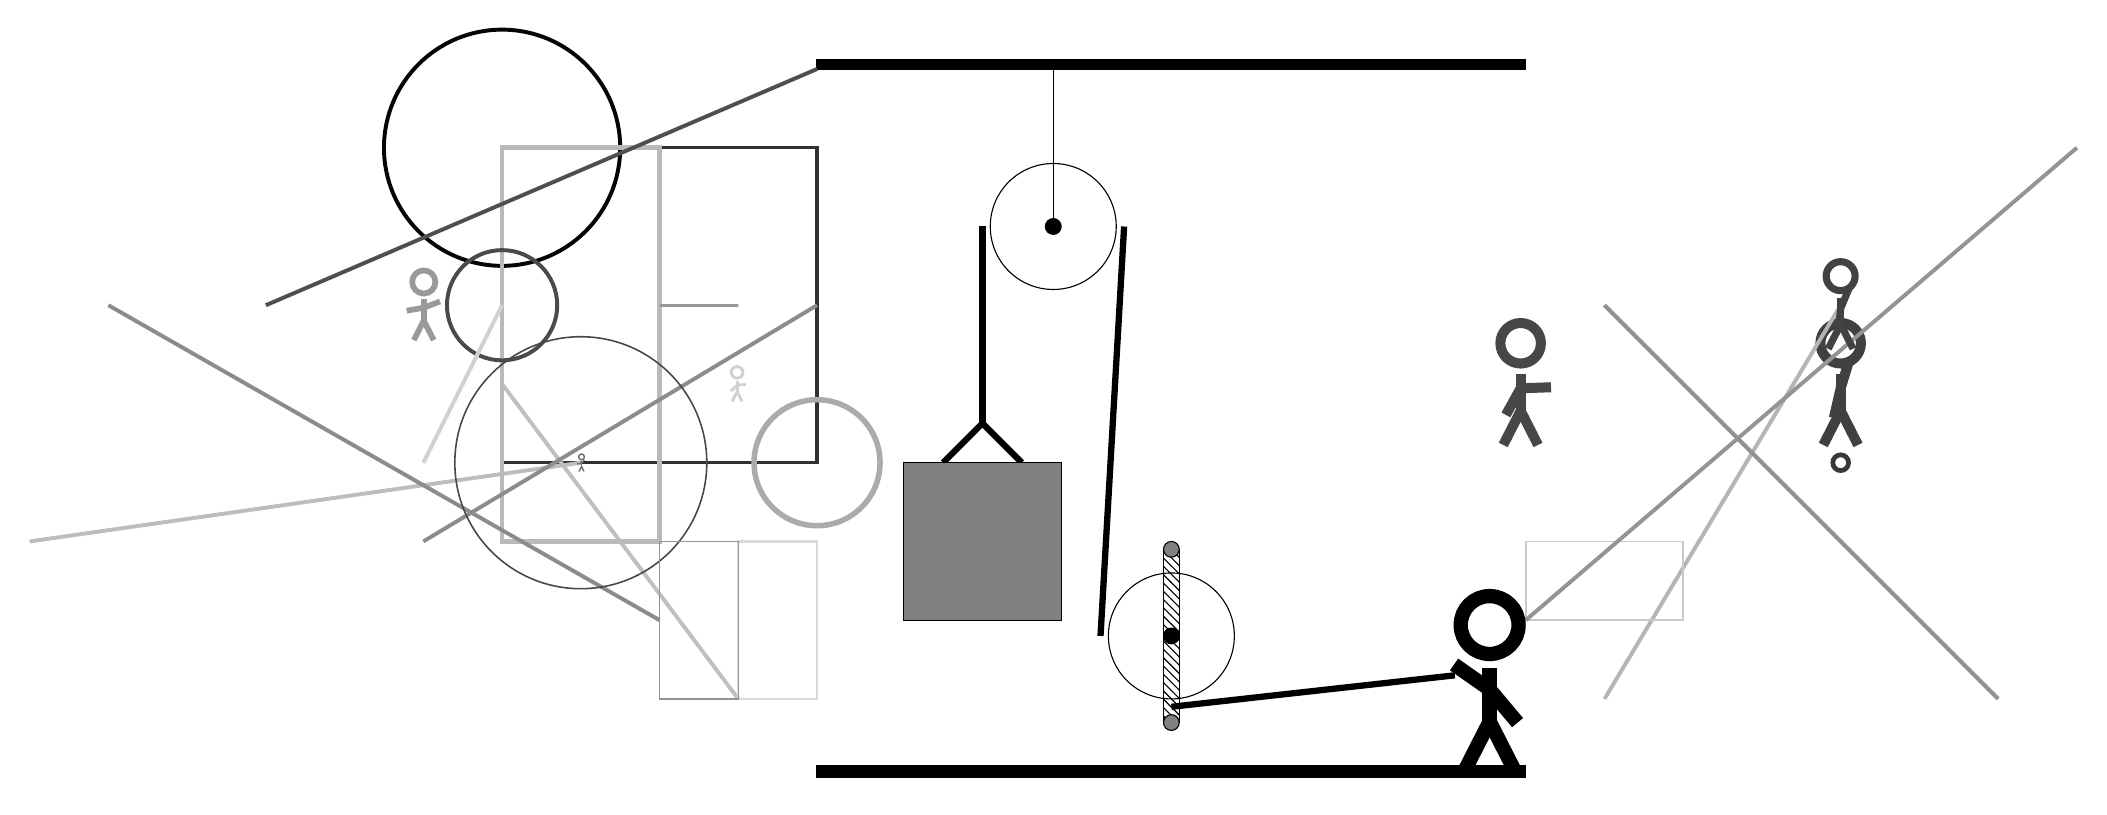
\begin{tikzpicture}
			%%%%% START %%%%%
			
			\draw[fill=black] (-2, 9) rectangle (7, 9.125);
			
			\draw (1, 7) circle (0.8);
			\draw[fill=black] (1, 7) circle (0.1);
			\draw (1, 9) -- (1, 7);
			
			\draw[line width=0.4mm, color=black!81] (-2, 8) rectangle (-6, 4);
			
			\node[line width=0.3mm, color=black!72] at (7, 5) {\Strichmaxerl[7][61][2]};
			\node[line width=0.2mm, color=black!75] at (11, 5) {\Strichmaxerl[7][77][73]};
			\draw[line width=0.5mm, color=black!29](11, 6) -- (8, 1);
			
			\draw [line width=0.7mm, color=black!33](-2, 4) circle (0.8);
			
			\draw [line width=0.6mm, color=black!78](11, 4) circle (0.1);
			
			\draw [line width=0.5mm, color=black!98](-6, 8) circle (1.5);
			\draw[line width=0.5mm, color=black!26](-5, 4) -- (-12, 3);
			\draw[line width=0.5mm, color=black!25](-6, 5) -- (-3, 1);
			\draw[line width=0.4mm, color=black!71] (-3, 7) rectangle (-3, 7);
			
			\draw[line width=0.2mm, color=black!21] (7, 2) rectangle (9, 3);
			\draw[line width=0.5mm, color=black!43](8, 6) -- (13, 1);
			\draw[line width=0.6mm, color=black!27] (-4, 3) rectangle (-6, 8);
			\draw [line width=0.5mm, color=black!71](-6, 6) circle (0.7);
			\draw[line width=0.3mm, color=black!15] (-3, 1) rectangle (-2, 3);
			\draw[line width=0.5mm, color=black!69](-2, 9) -- (-9, 6);
			
			\node[line width=0.6mm, color=black!57] at (-5, 4) {\Strichmaxerl[1][7][50]};
			
			\draw[line width=0.5mm, color=black!45](-4, 2) -- (-11, 6);
			\draw[line width=0.5mm, color=black!45](-2, 6) -- (-7, 3);
			\draw [line width=0.2mm, color=black!72](-5, 4) circle (1.6);
			\draw[line width=0.5mm, color=black!42](7, 2) -- (14, 8);
			\node[line width=0.3mm, color=black!40] at (-7, 6) {\Strichmaxerl[4][10][21]};
			\draw[line width=0.2mm, color=black!42] (-3, 1) rectangle (-4, 3);
			\node[line width=0.7mm, color=black!18] at (-3, 5) {\Strichmaxerl[2][43][5]};
			\node[line width=0.6mm, color=black!74] at (11, 6) {\Strichmaxerl[5][84][67]};
			
			\draw[line width=0.4mm, color=black!41] (-3, 6) rectangle (-4, 6);
			\draw[line width=0.5mm, color=black!18](-6, 6) -- (-7, 4);
			
			\draw[fill=white](2.5, 1.8) circle (0.8);
			\draw[fill=black] (2.5, 1.8) circle (0.1);
			\draw[pattern=north west lines, pattern color=black] (2.4, 2.9) rectangle (2.6, 0.7);
			\draw[fill=black!50] (2.5, 2.9) circle (0.1);
			\draw[fill=black!50] (2.5, 0.7) circle (0.1);
			
			\draw[line width=0.8mm] (-0.4, 4.0) -- (0.1, 4.5) -- (0.6, 4.0);
			\draw[fill=black!50] (-0.9, 4.0) rectangle (1.1, 2.0);
			
			\draw[line width=0.8mm] (0.1, 7) -- (0.1, 4.5);
			\centerarc[line width=0.8mm](1, 7)(0:180:0.9);
			\draw[line width=0.8mm](1.9, 7) -- (1.6, 1.8);
			\centerarc[line width=0.8mm](2.5, 1.8)(180:270:0.9);
			\draw[line width=0.8mm](2.5, 0.9) -- (6.1, 1.3);
			
			\node at (6.5, 1.2) {\Strichmaxerl[10][-35][-50]};
			
			\draw[fill=black] (-2, 0) rectangle (7, 0.15);
			
			%%%%% END %%%%%
		\end{tikzpicture}
	\end{figure}	
\end{document}